% Copyright 2004 by Till Tantau <tantau@users.sourceforge.net>.
%
% In principle, this file can be redistributed and/or modified under
% the terms of the GNU Public License, version 2.
%
% However, this file is supposed to be a template to be modified
% for your own needs. For this reason, if you use this file as a
% template and not specifically distribute it as part of a another
% package/program, I grant the extra permission to freely copy and
% modify this file as you see fit and even to delete this copyright
% notice. 

\documentclass{beamer}

% There are many different themes available for Beamer. A comprehensive
% list with examples is given here:
% http://deic.uab.es/~iblanes/beamer_gallery/index_by_theme.html
% You can uncomment the themes below if you would like to use a different
% one:
%\usetheme{AnnArbor}
%\usetheme{Antibes}
%\usetheme{Bergen}
%\usetheme{Berkeley}
%\usetheme{Berlin}
%\usetheme{Boadilla}
%\usetheme{boxes}
%\usetheme{CambridgeUS}
%\usetheme{Copenhagen}
%\usetheme{Darmstadt}
%\usetheme{default}
%\usetheme{Frankfurt}
%\usetheme{Goettingen}
%\usetheme{Hannover}
%\usetheme{Ilmenau}
%\usetheme{JuanLesPins}
%\usetheme{Luebeck}
\usetheme{Madrid}
%\usetheme{Malmoe}
%\usetheme{Marburg}
%\usetheme{Montpellier}
%\usetheme{PaloAlto}
%\usetheme{Pittsburgh}
%\usetheme{Rochester}
%\usetheme{Singapore}
%\usetheme{Szeged}
%\usetheme{Warsaw}

\title{Design and Implementation of OFDM System on FPGA}


\author{Seyed-Ehsan Koohestani}
% - Give the names in the same order as the appear in the paper.
% - Use the \inst{?} command only if the authors have different
%   affiliation.

\institute[PoliTo] % (optional, but mostly needed)
{

  Electronics and Telecommunications\\
  Politecnico di Torino
  }
% - Use the \inst command only if there are several affiliations.
% - Keep it simple, no one is interested in your street address.

\date{
Prof. Marina Mondin (PoliTo)\\
Prof. Roberto Garello (PoliTo)\\
Prof. Amir K. Khandani (uWaterloo)
}
% - Either use conference name or its abbreviation.
% - Not really informative to the audience, more for people (including
%   yourself) who are reading the slides online

\subject{Theoretical Computer Science}
% This is only inserted into the PDF information catalog. Can be left
% out. 

% If you have a file called "university-logo-filename.xxx", where xxx
% is a graphic format that can be processed by latex or pdflatex,
% resp., then you can add a logo as follows:

 \pgfdeclareimage[height=1cm]{university-logo}{logopolito-eps-converted-to.pdf}
 \logo{\pgfuseimage{university-logo}}

% Delete this, if you do not want the table of contents to pop up at
% the beginning of each subsection:
\AtBeginSubsection[]
{
  \begin{frame}<beamer>{Outline}
    \tableofcontents[currentsection,currentsubsection]
  \end{frame}
}

% Let's get started
\begin{document}

\begin{frame}
  \titlepage
\end{frame}

\begin{frame}{Outline}
  \tableofcontents
  % You might wish to add the option [pausesections]
\end{frame}

% Section and subsections will appear in the presentation overview
% and table of contents.
\section{Introduction}

\begin{frame}{What is OFDM?}
  \begin{itemize}
  
  \item {
\alert{Orthogonal Frequency Division Multiplexing} is a modulation format that is being used for many of the latest wireless and telecommunications standards.
  }
  
  \item {
OFDM is a form of multicarrier modulation. An OFDM signal consists of a number of closely spaced modulated carriers.
  }


  \item {
Any non-linearity in receiving system will cause interference between the carriers as a result of inter-modulation distortion.
  }

  \end{itemize}
\end{frame}

\begin{frame}{OFDM Characteristics}

OFDM advantages:
  \begin{itemize}
   
  \item {
Immunity to selective fading
  }
  
  \item {  
Resilience to interference
  }
  
  \item {  
Spectrum efficiency
  }
  
  \item {  
Resilient to ISI
  }
  
  \item {  
Resilient to narrow-band effects
  } 
  
   \item {  
Simpler channel equalisation
  }
  \end{itemize}

OFDM disadvantages:
  \begin{itemize}
   
  \item {
High peak to average power ratio
  }
  
  \item {  
Sensitive to carrier offset and drift
  }
   \end{itemize}
\end{frame}

\begin{frame}{Thesis Goals}{Motivation}
  \begin{itemize}
  
  \item {
Innovation in telecommunication concepts (Full-duplex communication, coding, etc); a standard platform is mandatory
  }
  
  \item {
Implement a basic OFDM architecture (IEEE 802.11a) receiver/ transmitter in the logic side
  }
  
  \item {  
Processor side (peripherals, memories, connection to the logic, etc)
  }
  
  \item {  
Bridge between the logic and processor (BRAM, AXI bus, DMA, etc)
  }
  
  \item {  
A evaluation board for RF side should be selected and initialize in software (power amplifiers, clock chains, ADC/ DAC)
  }
  
  \item {  
A correct methodology to test all the system elements together should be chosen
  }
  
     \end{itemize}
\end{frame}

\section{Theory, Design and Simulation}

\subsection{OFDM System Architecture}

\begin{frame}{Basic baseband OFDM system}
\begin{figure}[h!]
\centering
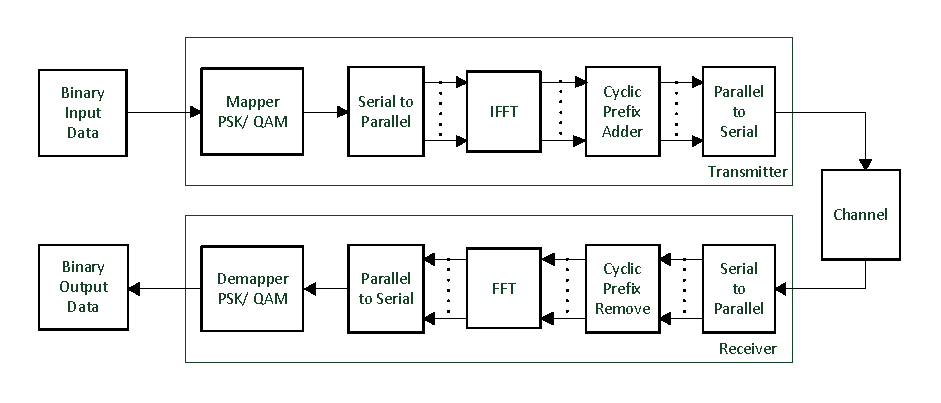
\includegraphics[width=\textwidth]{content/fig/basic_bb_ofdm.pdf}
\end{figure}
\end{frame}

\begin{frame}{Architecture of an OFDM system}
\begin{figure}[h!]
\centering
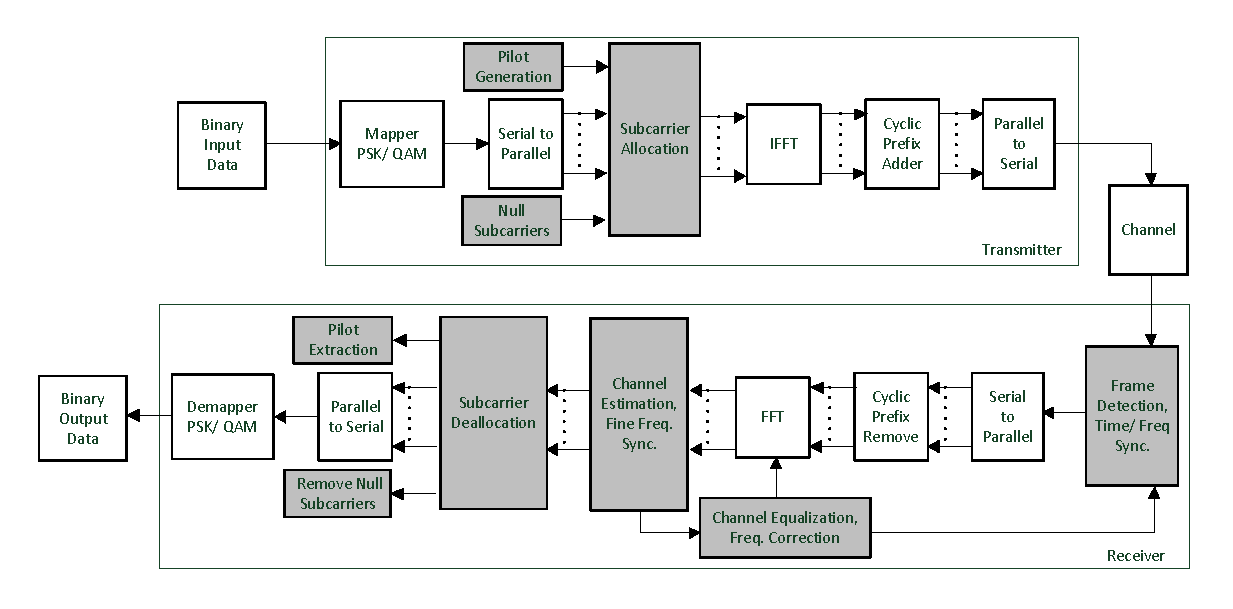
\includegraphics[width=\textwidth]{content/fig/practical_bb_ofdm.pdf}
\end{figure}
\end{frame}

\begin{frame}{Basic Parameters}
  \begin{itemize}
   
  \item {
Delay spread expected for the channel ($300 ns$)
  }
  
  \item {  
Guard duration ($800 ns$) which describes symbol duration ($4.0 \mu s$)
  }
  
  \item {  
Available bandwidth
  }
  
  \item {  
Data rate
  }

  \item {  
Number of Subcarriers 64 in 20 MHz
  }  

  \item {  
Roll-off factor $\beta$= 0.02
  }  
  
  \end{itemize}
\end{frame}

\begin{frame}{System parameters defined for the proposed design}
\begin{table}
\begin{tabular}{c|c|c}
Parameter&Description&Value\\ \hline
$B_{w}$&Available channel bandwidth&$20MHz$\\
$\sigma_{\tau}$&Delay spread of the channel& $<300 ns$\\
$T_{g}$&Guard interval duration (Cyclic Prefix)&$0.8\mu s$\\
$T_{sym}$&OFDM symbol period&$4.0\mu$\\
$T$&Effective symbol duration (FFT period)&$3.2\mu s (=T_{g}- T_{sym})$\\
$\Delta f$&Subcarrier spacing&$312.5kHz (=1/T)$\\
$N_{g}$&Number of guard samples&$16$\\
$N$&FFT size&$64= B/\Delta f s$\\
$N_{d}$&Number of data subcarriers&$48$\\
$N_{p}$&Number of pilot sucarriers&$4$\\
$N_{u}$&Number of used subcarriers&$52$\\
$B_{u}$&Signal occupied bandwidth&$16.6MHz$\\
$R_{b}$&Data rate without coding&$12Mbps, 24Mbps$\\
\end{tabular}
\end{table}
\end{frame}

\begin{frame}{Bit Error Rate}

Theoretical equation of the BER for a QPSK:
\begin{equation}
P_{b}(e)= \dfrac{1}{2}erfc(\sqrt{\dfrac{E_{b}}{N_{0}}})
\end{equation}

Non-ideality :
\begin{equation}
P_{b}(e)= \dfrac{1}{2}erfc(\sqrt{\dfrac{E_{b}}{N_{0}}\dfrac{T}{T+T_{g}}\dfrac{N_{u}}{N_{u}+N_{p}}})
\end{equation}

Replacement:
\begin{equation}
P_{b}(e)= \dfrac{1}{2}erfc(\sqrt{\dfrac{E_{b}}{N_{0}}0.65})
\end{equation}


\end{frame}

\begin{frame}{Preamble of IEEE 802.11}

\begin{figure}[h!]
\centering
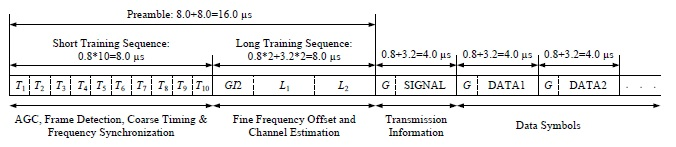
\includegraphics[width=\textwidth]{content/fig/ofdm_frame.JPG}
\end{figure}
\end{frame}


\begin{frame}{Design Block Diagram of OFDM PHY}

\begin{figure}
\centering
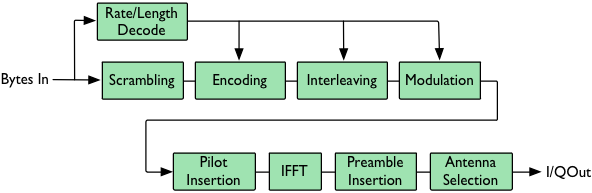
\includegraphics[width=10cm]{content/fig/wlan_phy_tx_blk_diag.png}
\end{figure}

\begin{figure}
\centering
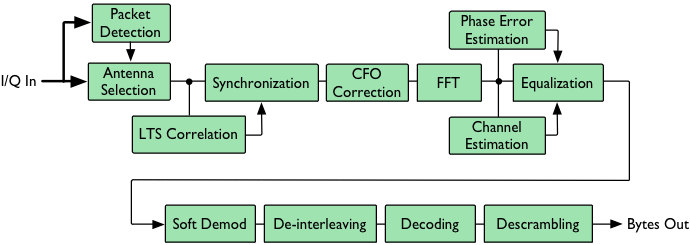
\includegraphics[width=10cm]{content/fig/wlan_phy_rx_blk_diag.png}
\end{figure}

\end{frame}


\begin{frame}{General models of a direct conversion RF}
\begin{figure}[h!]
\centering
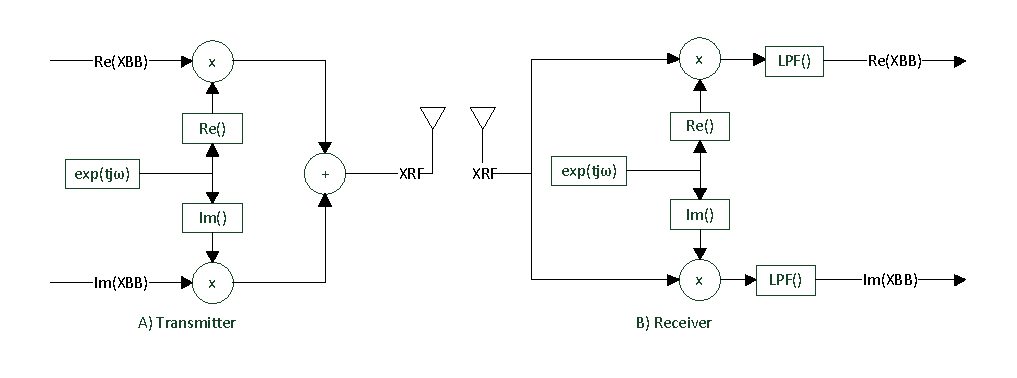
\includegraphics[width=10cm]{content/fig/drct_rf_mdl.pdf}
\end{figure}

  \begin{itemize}
   
  \item {
Phase offset across subcarriers in an symbol which can be  estimated by pilot tones and corrected in frequency domain  
}
  
  \item {  
Degradation of orthogonality between subcarriers in receiver's FFT which causes inter-carrier interference (ICI)
  }
  
  \end{itemize}
  
\end{frame}

\begin{frame}{OFDM performance loss due to CFO-induced ICI}
\begin{figure}[h!]
\centering
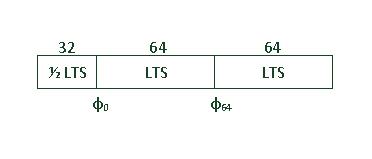
\includegraphics[width=5cm]{content/fig/lts_time_domain.pdf}
\end{figure}

\begin{equation}
\begin{split}
CFO \approx (\phi_{64}- \phi_{0})\\
CFO_{EST} = \frac{f_{s}}{2\pi . 64^{2}} \sum\limits_{n=64}^{127} \phi_{n}- \phi_{(n-64)}\\
\end{split}
\end{equation}

\begin{figure}[h!]
\centering
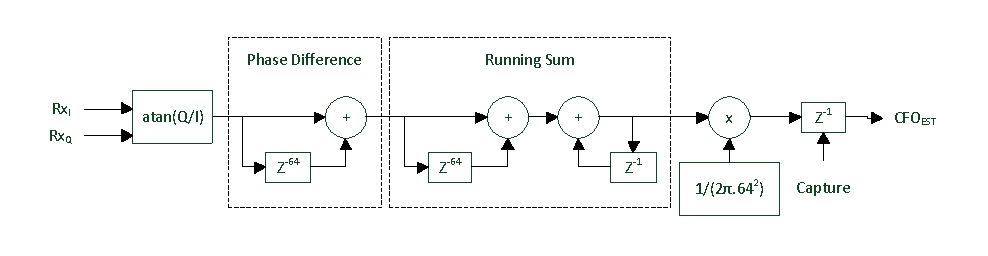
\includegraphics[width=10cm]{content/fig/time_dom_cfo_est.pdf}
\end{figure}

\end{frame}

\begin{frame}{Synchronization}

Cross-Correlation
\begin{equation} \label{P_n}
P(n) = \sum\limits_{m=0}^{L-1} r_{n+m} r^{*}_{n+m+D}
\end{equation}
Auto-Correlation
\begin{equation} \label{R_n}
 R(n) = \sum\limits_{m=0}^{L-1} r_{n+m+D} r^{*}_{n+m+D}
\end{equation}

Schimdl and Cox Delay and Correlate Algorithm
\begin{figure}[h!]
\centering
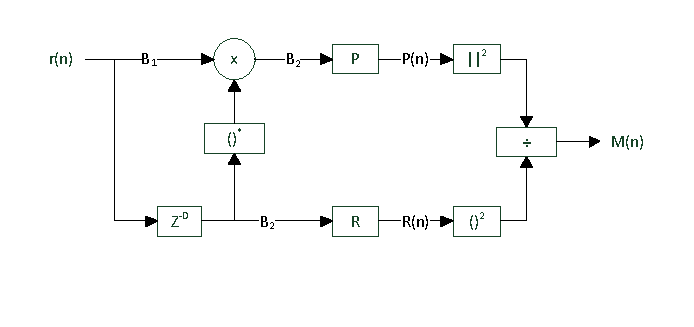
\includegraphics[width=10cm]{content/fig/schl_cox_mdl.pdf}
\end{figure}
\end{frame}

\subsection{Hardware Implementation}

\begin{frame}{System Generator Cycle}
\begin{figure}[h!]
\centering
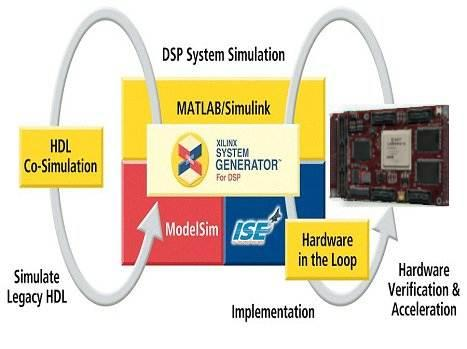
\includegraphics[width=5cm]{content/fig/systemGen.JPG}
\end{figure}
\begin{figure}[h!]
\centering
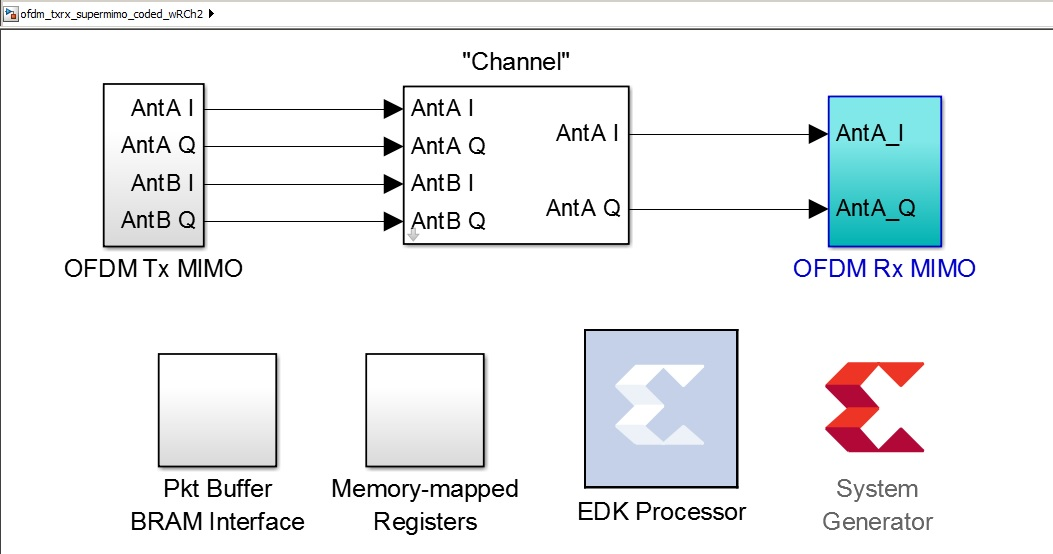
\includegraphics[width=5cm]{content/fig/system.JPG}
\end{figure}
\end{frame}


\begin{frame}{System Generator Sample}

OFDM Receiver Block
\begin{figure}
\centering
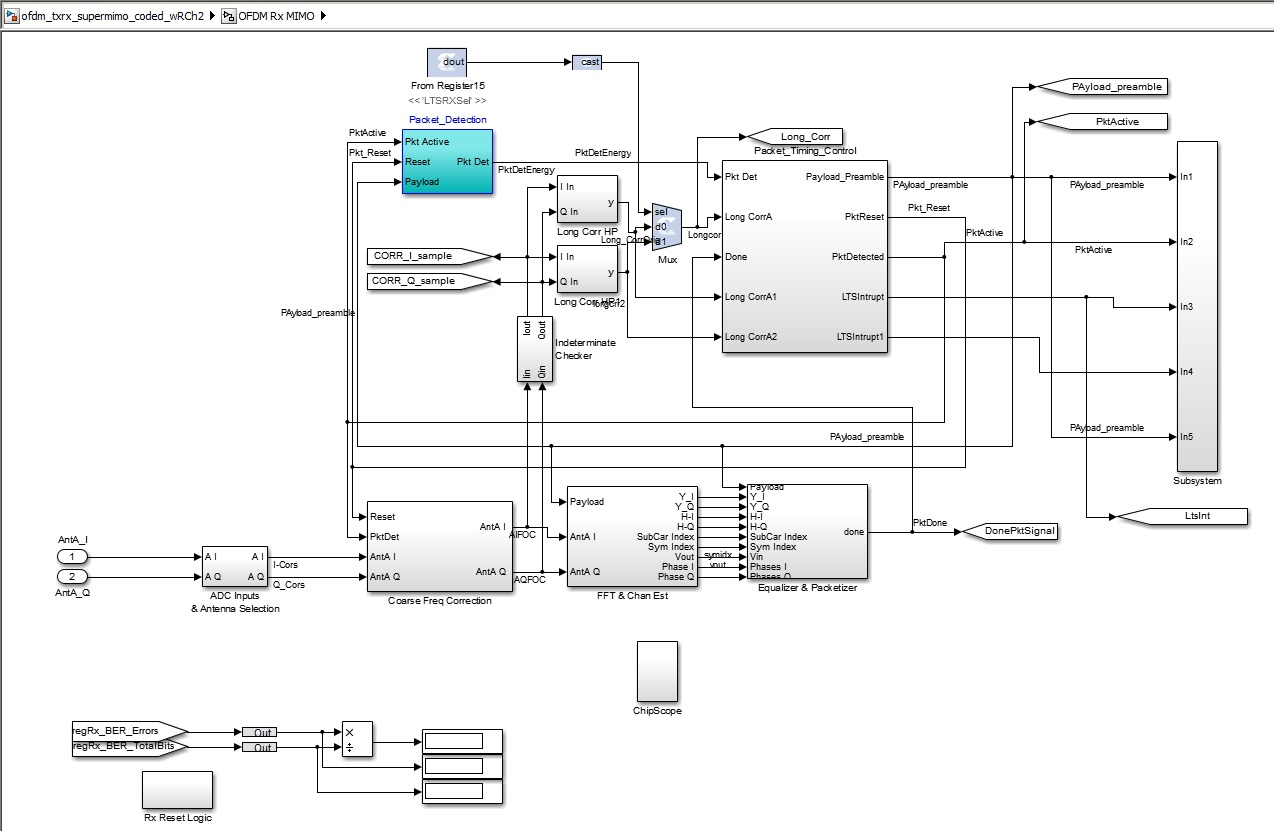
\includegraphics[width=10cm]{content/fig/rxblock.JPG}
\end{figure}
\end{frame}

\begin{frame}{Radio Board} {AD-FMCOMMS1-EBZ}
\begin{figure}
\centering
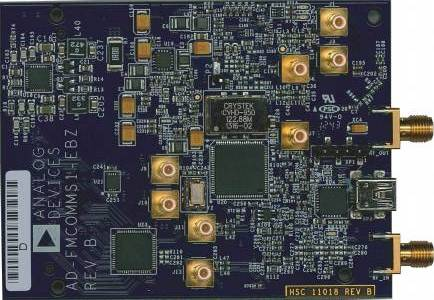
\includegraphics[width=3cm]{content/fig/fmcomms1.jpg}
\end{figure}

\begin{figure}
\centering
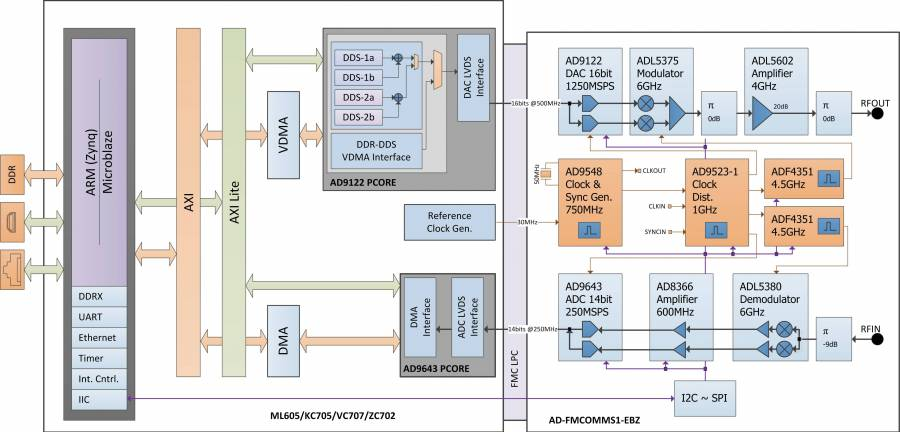
\includegraphics[width=10cm]{content/fig/fmcomms1Blockdiagram.jpg}
\end{figure}
\end{frame}

\begin{frame}{Board Elements}
  \begin{itemize}
   
  \item {
Clock chain is re-programmed based on our necessities in the FPGA architecture design
  }
  
  \item {  
Clock synchronization blocks are studied to be in our design margin
  }
  
  \item {  
Non-linearity caused by the modems, amplifiers and ADC/DAC are studied 
  }
  
   \end{itemize}
\end{frame}

\begin{frame}{OFDM on FPGA?}
  \begin{itemize}
   
  \item {
Flexibility, re-configurable
  }
  
  \item {  
Parallel processing
  }

  \item {  
Re-use of the processing units (FFT, filters, etc)
  }
  
  \item {  
Triangle operations are not easy to implement!
  }
  
  \item {  
A processor on standard communication ports (UART, I2C, Ethernet) 
  }
  
    \item {  
Reliable bridge between logic side and processor side 
  }
  
   \end{itemize}
\end{frame}

\begin{frame}{Design Block Diagram}{Full Design with Processor}
\begin{figure}
\centering
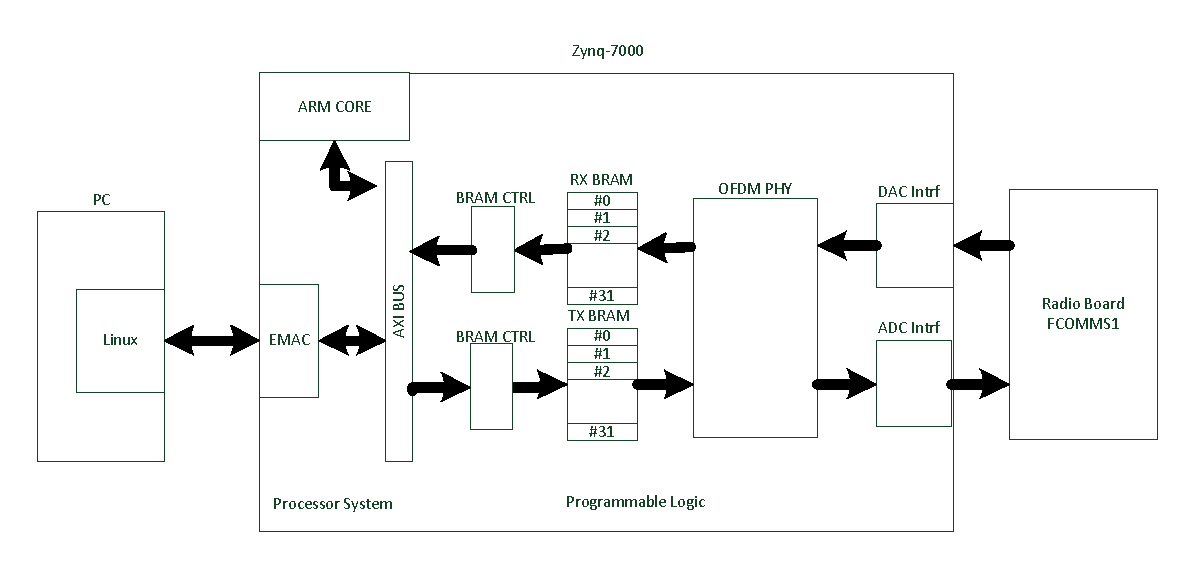
\includegraphics[width=\textwidth]{content/fig/sys_block_diagram.pdf}
\end{figure}
\end{frame}

\begin{frame}{Hardware set-up}
\begin{figure}
\centering
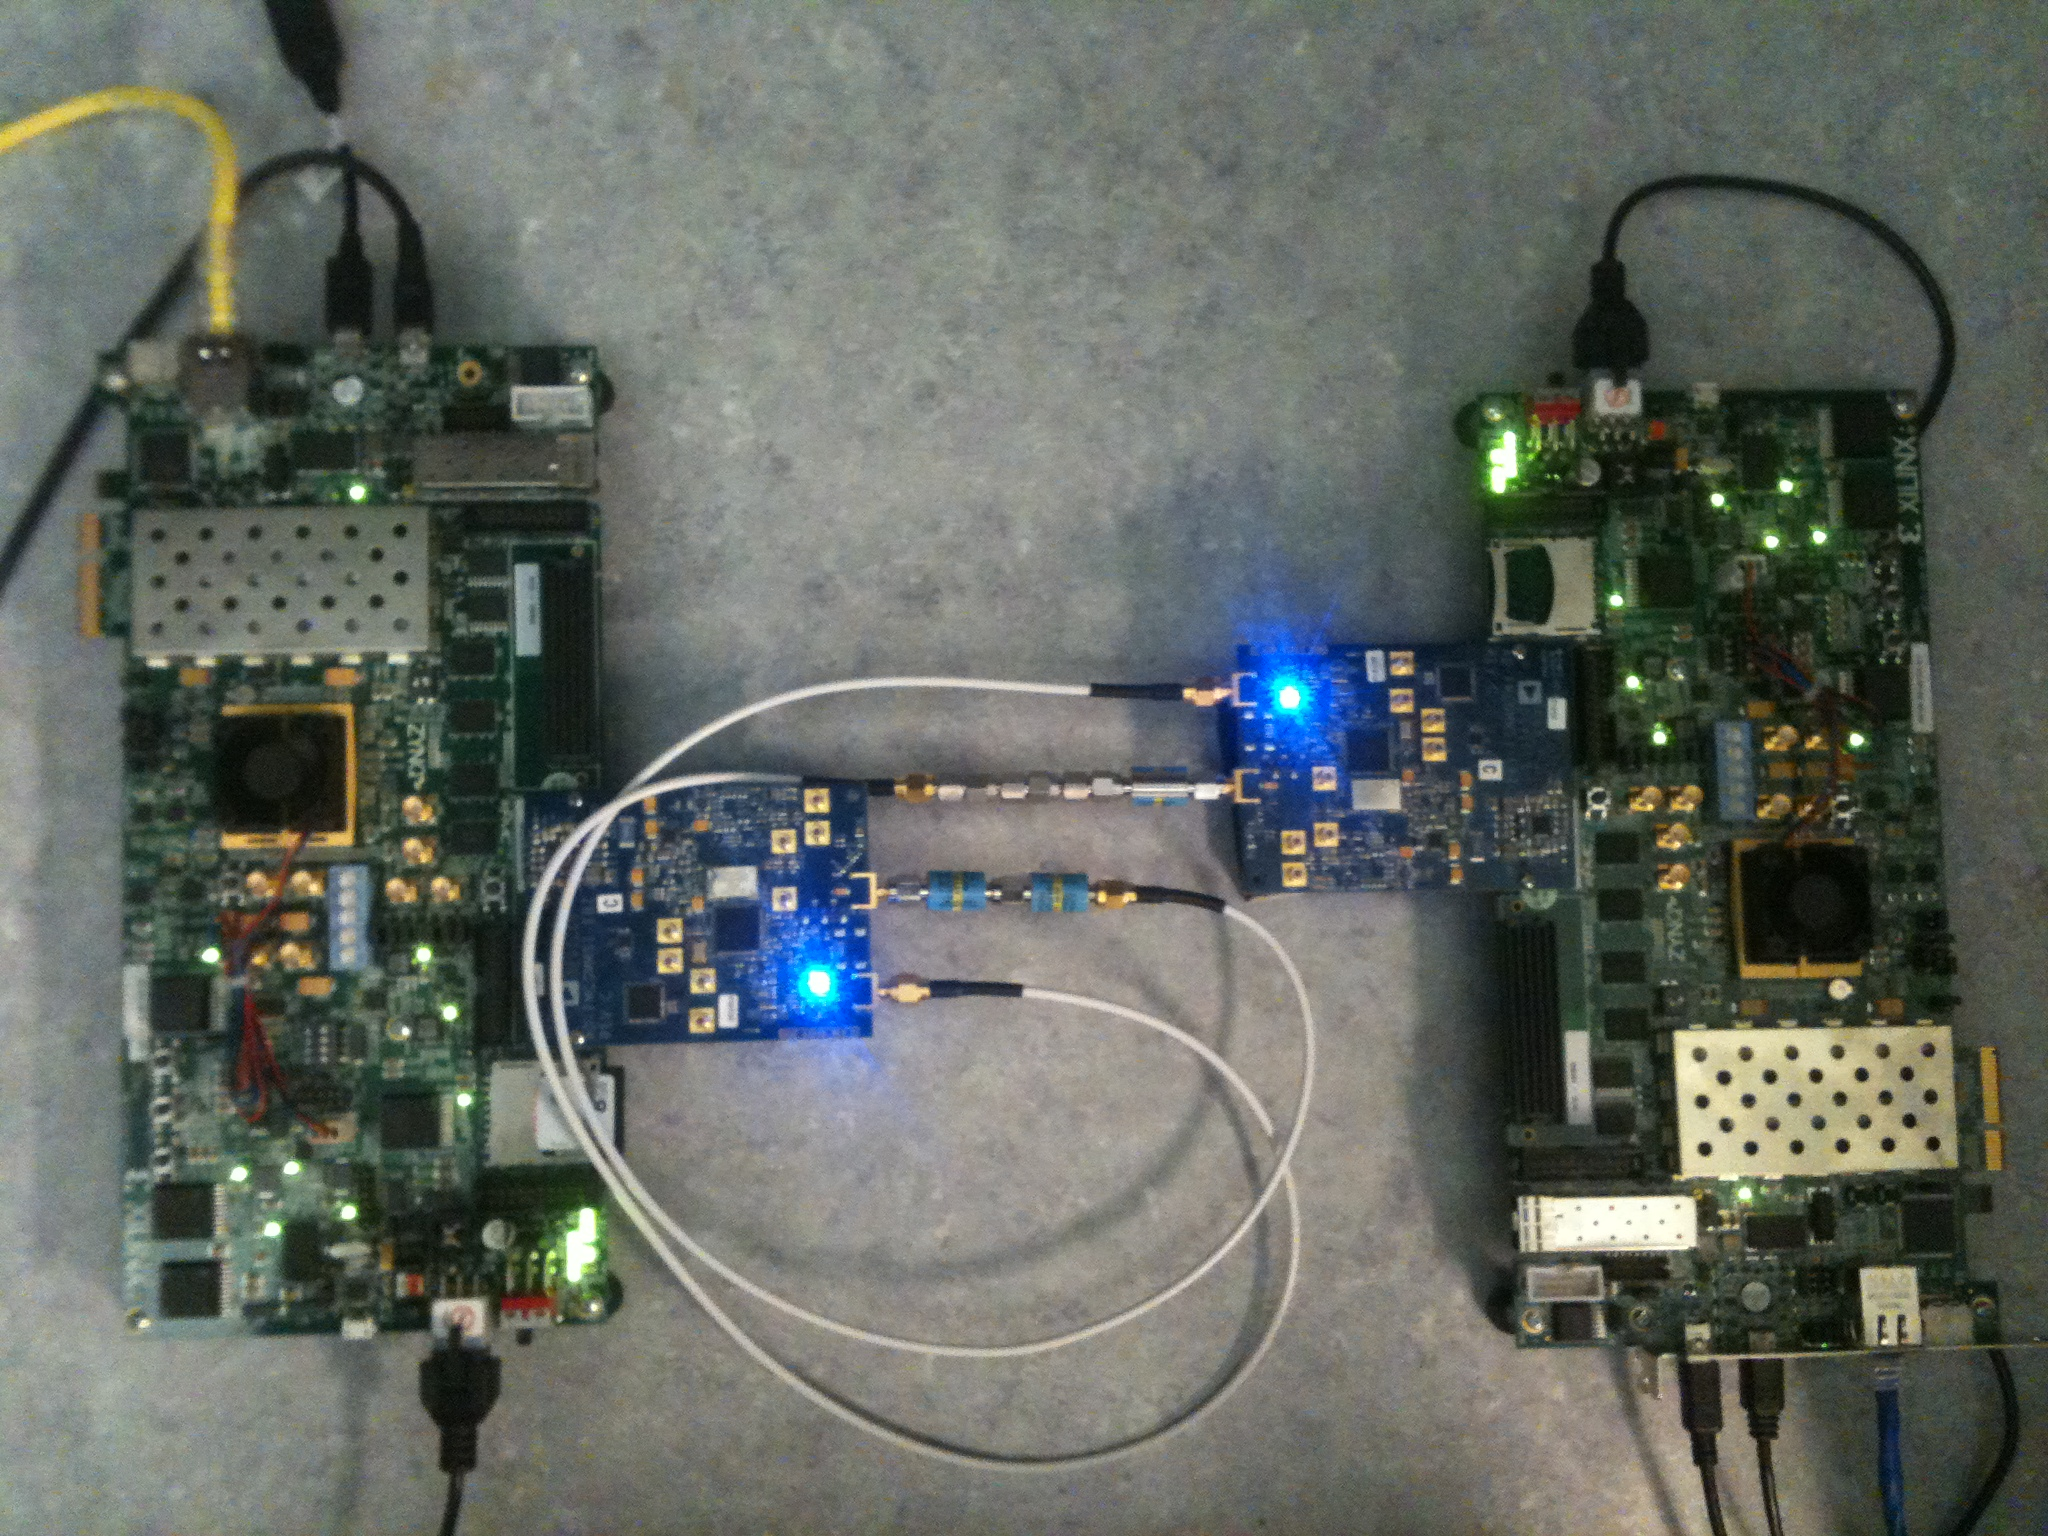
\includegraphics[width=10cm]{content/fig/hardware_setup.JPG}
\end{figure}
\end{frame}

\section{Sample Analysis and Conclusion}

\subsection{Hardware Samples and Analysis}

\begin{frame}{OFDM Frame (I/Q) detected in Chipscope}
\begin{figure}
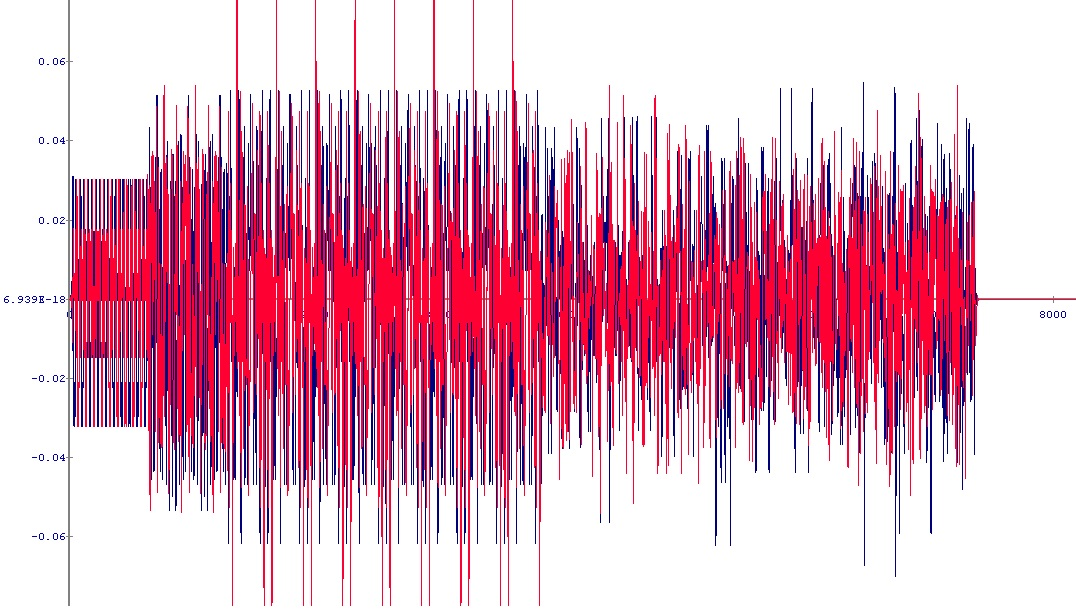
\includegraphics[width=\textwidth]{content/fig/ofdmframe_chipscope.JPG}
\end{figure}
\end{frame}

\begin{frame}{Chipscope samples}

Cross Correlation on LTS \hspace{20 mm} Auto Correlation on STS
\begin{figure}
\centering
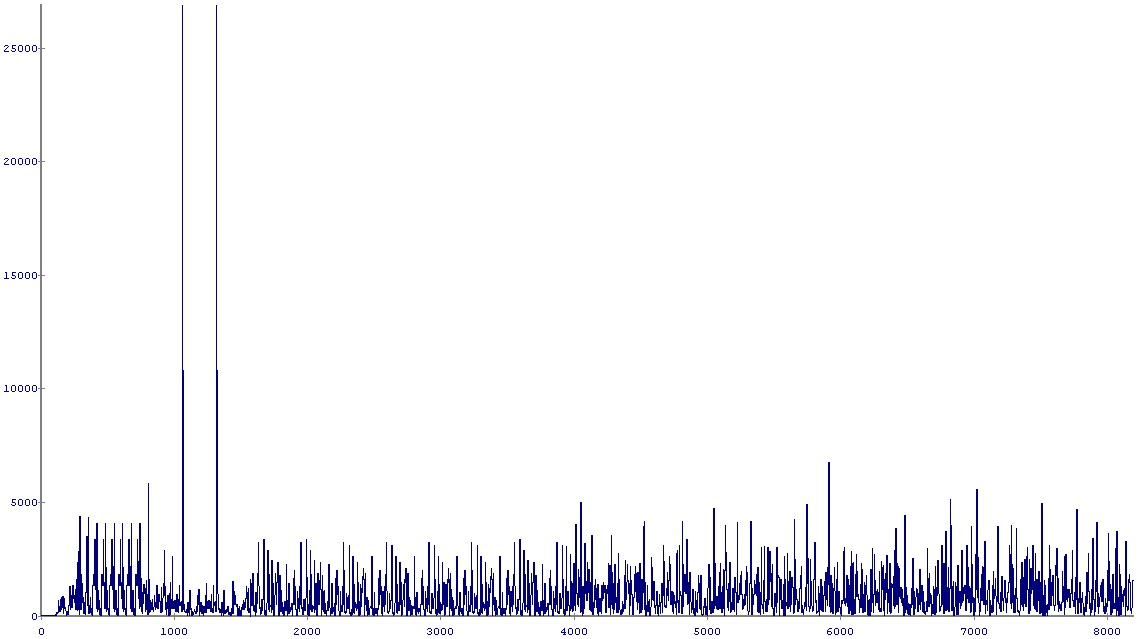
\includegraphics[width=6cm]{content/fig/crosscorr.JPG}
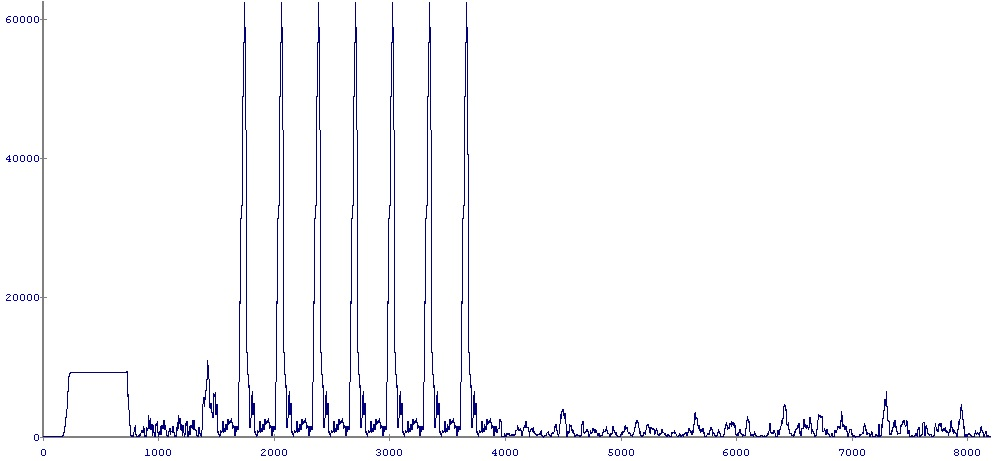
\includegraphics[width=7cm]{content/fig/autocorr.JPG}
\end{figure}
\end{frame}

\begin{frame}{LTS Spectrum- passed RF chain}
\begin{figure}
\centering
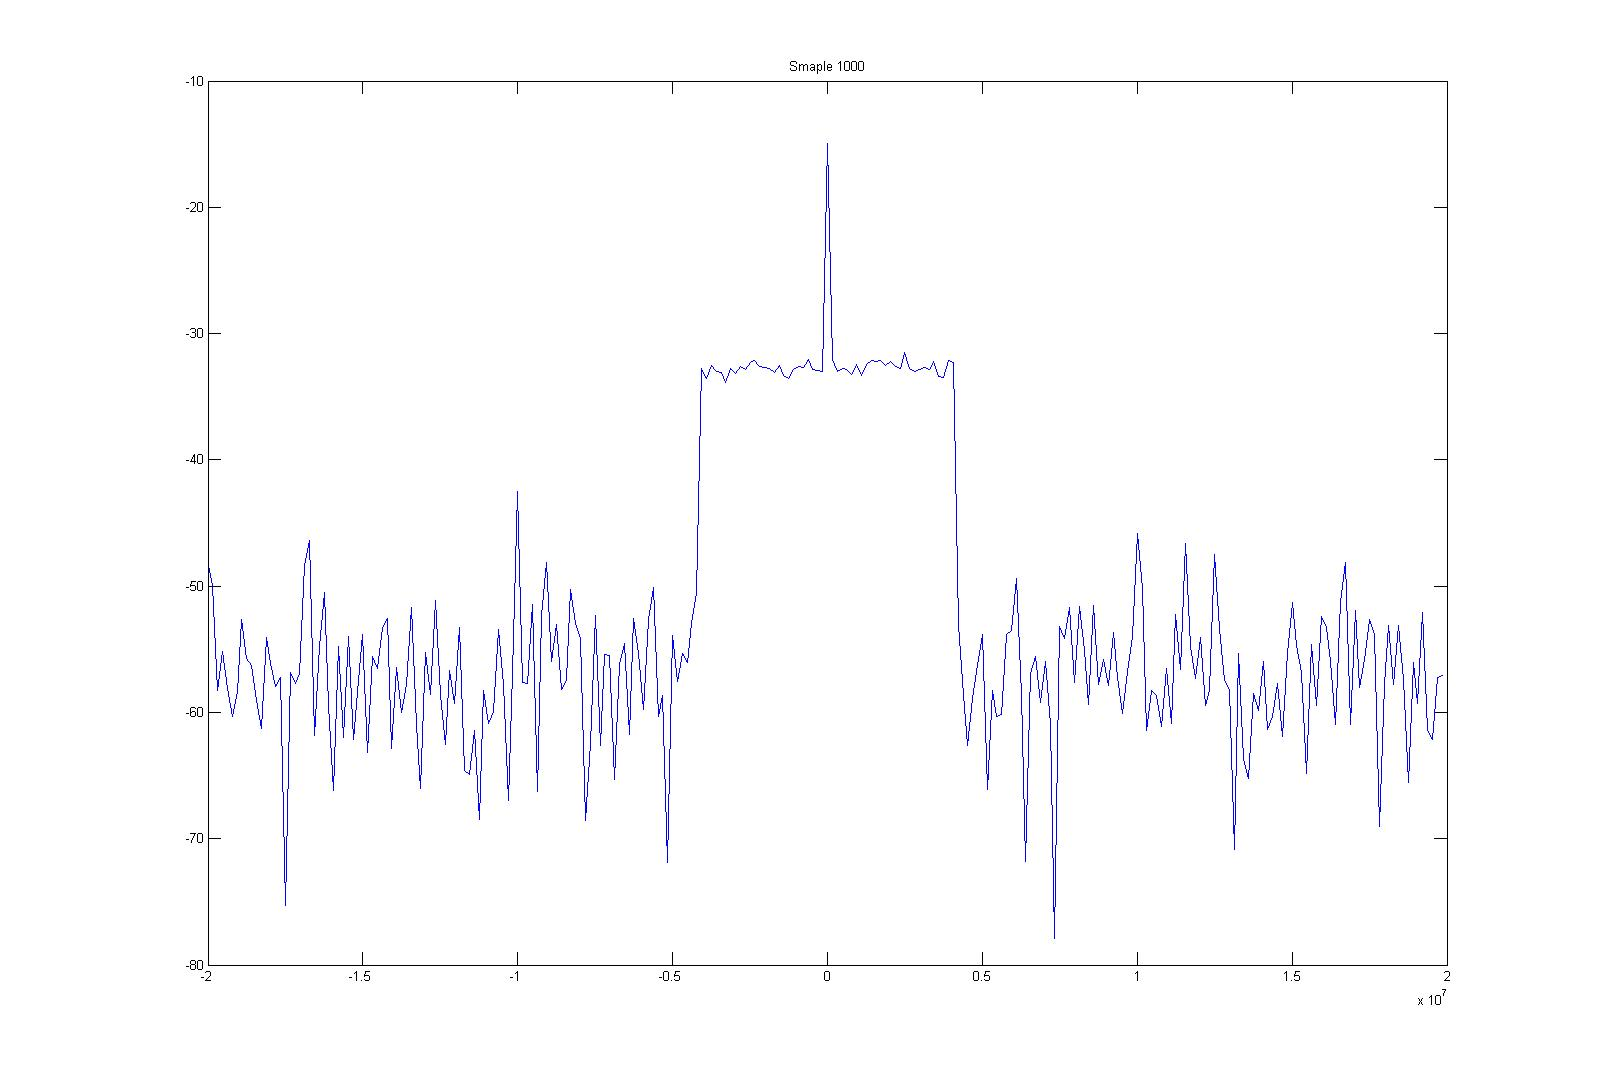
\includegraphics[width=10cm]{content/fig/Rfbase.JPG}
\end{figure}
\end{frame}

\begin{frame}{Device Utilization Summary }{XC7Z045-22FFG900C}

\begin{table}
\centering
\vspace{0.5cm}
\begin{tabular}{c|c|c|c}
Slice Logic Utilization&Used&Available&Utilization\\ \hline
Number of Slice Registers&42,703&437,200&9\% \\
Number of Slice LUTs&59,787&218,600&27\% \\
Number used as Memory&5,384&70,400&7\% \\
Number of occupied Slices&21,749&54,650&39\% \\
Number of DSP48E1s&149&900&16\% \\
\end{tabular}
\end{table}

\end{frame}


% Placing a * after \section means it will not show in the
% outline or table of contents.
\section*{Summary}

\begin{frame}{Summary}
  \begin{itemize}
  \item
   The OFDM system is prototyped based on IEEE 802.11a standard and transmits/receives signals on a 20 MHz bandwidth (throughput of 24 Mbps).
  \item
    System Generator is not optimized. There are low-level techniques to manage the power, speed and area.
  \end{itemize}
  
\end{frame}

\begin{frame}
\centering
   Thanks for your attention.

\end{frame}

\end{document}


